\chapter{Methods and Analysis chapter}

% Take my thesis and copy the style, however, basically what you did and how you did it 
% So 
% \begin{itemize}
%     \item Each method \& analysis has its section
%     \item Draw some conclusions about this (here \textbf{technical} ones!)
% \end{itemize}

% CHAPTER SCHEMA
% - what is a graph formally                DONE 
% - visualization methods, layouts, not interesting geographically + global overview
%     - how the force directed works
% - centrality measures:
%     - degree (abs/perc) (in/out) (weight/unw) 
%         - (1-inw: vulnerability)
%         - power law (degree/in/out)(unw/weight)
%     - why not betweenness and closeness
%     - density
%     - clustering
%     - page rank
% - community measures:
%     - sbm
%     - louvain

Adapted from \textcite{barabasi2016network,easley2012networks}.

\section{Intro to Graph Theory}

If we want to understand a complex system, we first need to know how its components interact with each other or, in other words, we need a map of its wiring diagram.
Let us start by defining formally what is a graph, since it is fundamental for the analysis that will be carried out. 
A \textit{graph} is a way of specifying relationships among a collection of items. It consists of a set of objects, called \textit{nodes}, with certain pairs of these objects connected by links called \textit{edges}. If we denote by $\mathcal{N}$ the set of nodes, and $\mathcal{E}$ the set of edges, then they are sufficient to identify a graph 
\[ \mathcal{G} = (\mathcal{N},\mathcal{E})\,. \]
We say that two nodes are \textit{neighbors} if they are connected by an edge. This representation of the network offers a common language to study systems that may differ greatly in nature or scope. The links of a graph can be \textit{directed} or \textit{undirected}: some systems have directed edged, such as the world trade of goods that we analyze in this research where a country imports from another country and the transit of goods has a clear direction, while other systems have undirected edges, like friendship relationships in a social community, where the connection between the entities is mutual (if I am your friend then you are my friend).

A complete description of a graph requires us to keep track of its nodes and edges: this is often done using a so-called \textit{adjacency matrix}. The adjacency matrix $A$ of a directed graph with $N$ nodes is a $N \times N$ matrix, where $A_{ij} = 1$ if there is an edge going from node $j$ to node $i$, while $A_{ij} = 0$ if there isn't. For an undirected network instead, the adjacency matrix has the property of being symmetric, i.e. $A_{ij} = A_{ji}$.

Another relevant distinction about graphs is whether the edges have a weight assigned to them or not. A network is called \textit{weighted} if each edge $(i,j)$ has a unique weight $w_{ij}$ assigned to it. It is called \textit{unweighted} (or \textit{binary}) if it has no weights assigned, or equivalently if the possible weights are just $\{0,1\}$ (no edge vs. edge). For the \textit{weighted} networks the elements of the adjacency matrix contain the weight of the edges as $A_{ij} = w_{ij}$. This is the case with the trade networks that we are going to analyze, where the edges between two countries have as weight the monetary value of the exchange.


\paragraph{Node properties.}
A key property of each node is its \textit{degree}, which is the number of edges that it has to other nodes. We denote by $k_i$ the degree of the $i$-th node in the graph. In our specific case, the degree of a node represents the number of commercial partners that a country has, for either import or export: for example, Italy had a degree of (TODO:insert italy degree) in YYYY, meaning that it traded goods with X partners in that year.
Since the network under consideration is directed, we make a distinction between \textit{incoming degree} (or \textit{in-degree}) and \textit{outgoing degree} (or \textit{out-degree}):
\begin{itemize}
    \item \textit{in-degree}: denoted by $k_i^{in}$, is the number of edges that point to node $i$;
    \item \textit{out-degree}: denoted by $k_i^{out}$, is the number of edges that point from node $i$ to other nodes.
\end{itemize}
The degree $k_i$ of node $i$ can be directly obtained from the elements of the adjacency matrix: if the network is undirected, summing over the rows (or the columns) gives in return a vector of all the node degrees. For a directed network instead, the two sums give different metrics: the sum over the rows gives the incoming degrees, while the sum over the columns the outgoing degrees.

Given all the degrees of the nodes in the graph, one can also introduce the \textit{degree distribution} $p_k$, which is a discrete distribution indicating the probability that a randomly selected node has degree $k$. For a network of $N$ nodes, the degree distribution is the normalized histogram given by 
\[ p_k = \frac{N_k}{N} \]
where $N_k$ is the number of nodes that have degree $k$. \\

TODO: insert piece about weighted degree (strength) \\

The \textit{clustering coefficient} represents the extent to which the neighbors of a given node are linked to each other. For a node $i$ with degree $k_i$ the local clustering coefficient is
\[
    C_i = \frac{2 L_i}{k_i(k_i-1)}
\]
where $L_i$ is the number of edges among the $k_i$ neighbors of node $i$.
The clustering coefficient measures the graph's local edge density: in fact, the more interconnected the neighborhood of node $i$ is, the higher the coefficient.

\paragraph{Graph properties.}
Aside from looking at the node degrees one by one, one can also combine them to learn an important property of the graph as a whole, that is the \textit{average degree}. For an undirected network of size N the average degree is 
\[ k_{avg} = \frac{1}{N}\sum_{i=1}^N k_i = \frac{2 L }{N} \]
where $L = 1/2 \sum_{i=1}^N k_i$ is the total number of edges in the graph. If instead we consider a directed graph, we have that the average degree can be computed equivalently either using the in-degrees or the out-degrees
\[
    k_{avg}^{in} = \frac{1}{N} \sum_{i=1}^N k_i^{in} = \frac{1}{N} \sum_{i=1}^N k_i^{out} = k_{avg}^{out}\,,
\]
since the total number of links $L$ is the same if we sum either measures, \textit{in} or \textit{out}.
A second metric that we can compute for the whole network is the \textit{average clustering coefficient}, which represents the degree of clustering of the whole network:
\[
    C_{avg} = \frac{1}{N} \sum_{i=1}^N C_i
\]

\pagebreak
\section{Visualization of Trade Networks}

As it was previously shown in Section \ref{sec:ch3graphs} through the graph plots, a lot of insights and information can be gained through the visualization of the network. If we restrict our attention to the datasets and the tables, we can have an idea of the countries that play a major role in the global trade, and we receive the impression of the significance of the economic exchanges. However, we struggle to have a comprehensive view of the effects of these interactions on each other: for this reason, we make use of a graph which is able to capture and represent this type of intricate relationships. In order to do so, we need to spend special attention to how we display a graph, so that we can convey meaningful information. Since we are dealing with countries and imports, the most natural way to represent a world graph would be to use the geographical information of each nation: we collocate each node on the coordinates of the centroid of that country, and then we add the links among the countries (Figure \ref{fig:geograph}).
\begin{figure}
    \centering
    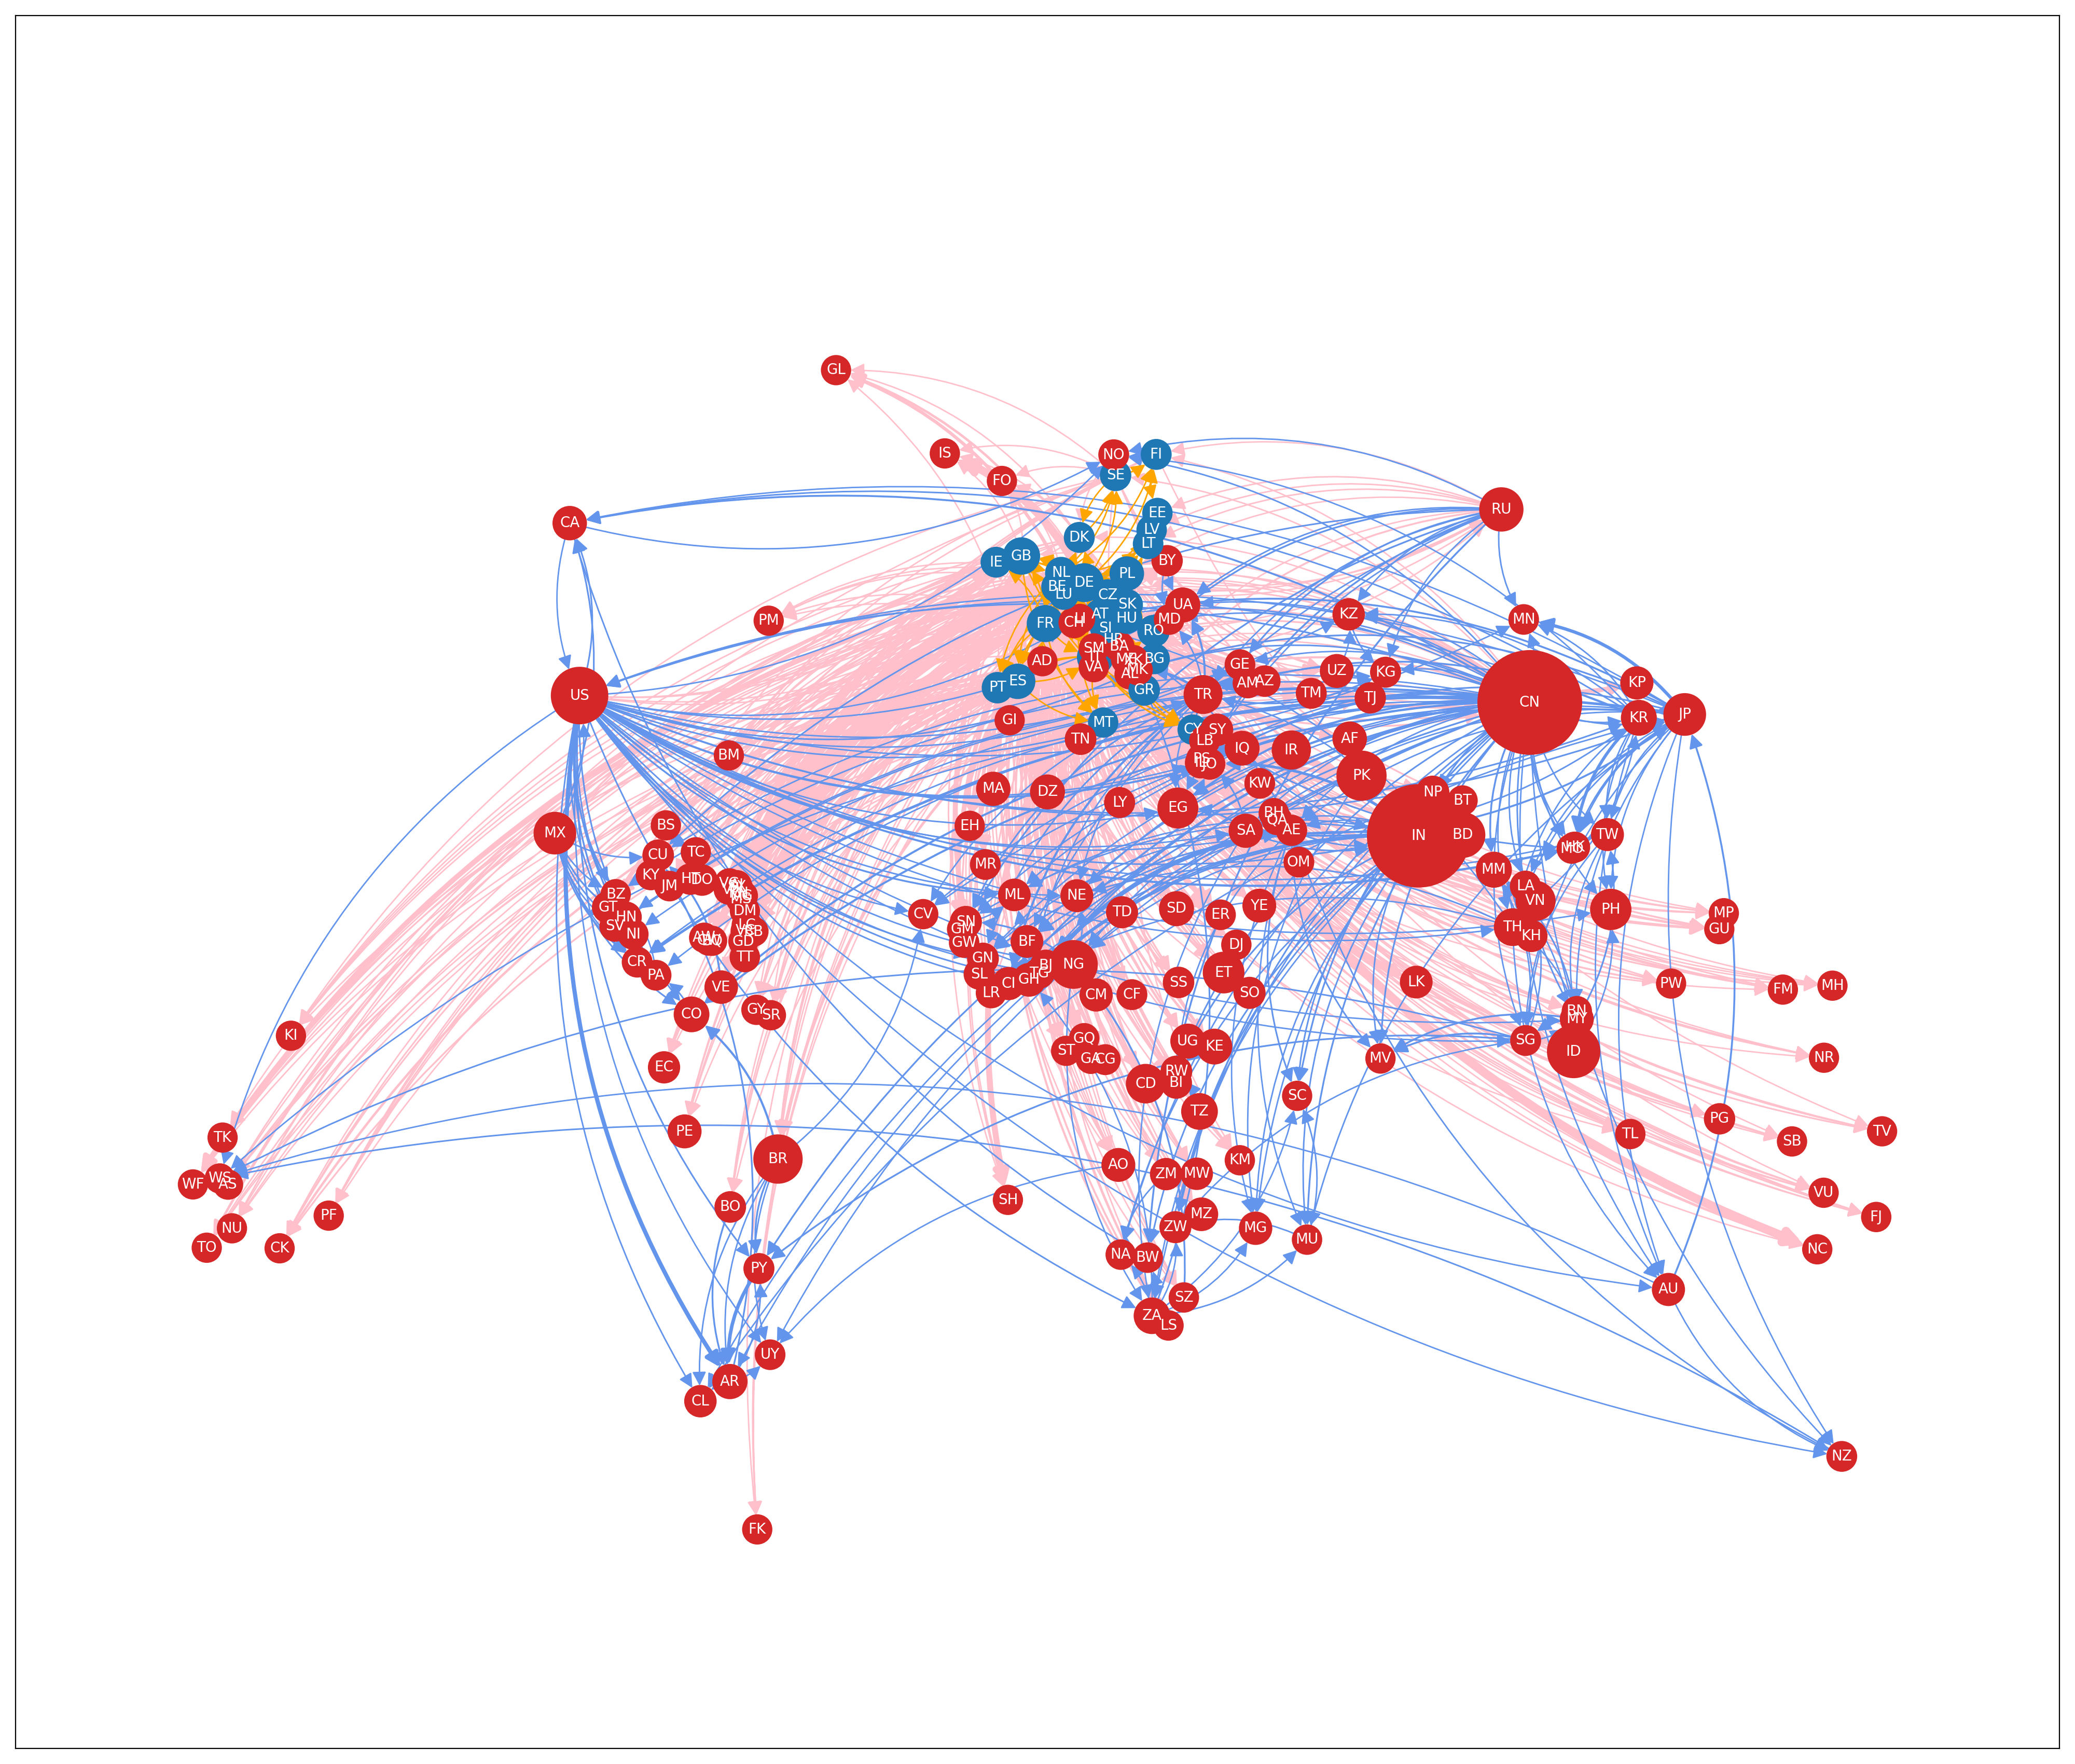
\includegraphics[width=\textwidth]{pics/full_y19_pTO_geo.png}
    \caption[Global trade network of all products in 2019.]{Global trade network of all products in 2019. Nodes are positioned according to the geographical location of the country, and their size is proportional to the population. The color of the node indicates EU countries (\textit{blue}) and non-EU (\textit{red}); the color of the edge is \textit{orange} for intra-EU exchanges, \textit{pink} for EU - non-EU exchanges and \textit{azure} for extra-EU exchanges. Only the top 5 import partnership for each country are shown.}
    \label{fig:geograph}
\end{figure}
What we can see in this plot is the complex net of trade routes among countries all around the world, and it emerges the important role that the greatest economies such as the US and China play in the global scenario. On the contrary, since all the blue nodes belonging to the European Union are so close to each other, it is impossible to see the web of intra-EU exchanges. What \textcite{benedictis2014bacicepii} point out, in fact, is that this picture does not give full account of the implication of the interdependence among countries, and using geographical positions we can draw conclusions only about the bilateral trades of countries, not their ensemble. In their words, ``\textit{this is the visual analog of the assumption of conditional independence among dyads imposed on international trade flows}".
If we want countries' interactions to be accounted in determining the relative position of each nation in the whole trading network, we should ignore their geographical position and move from a physical space to a \textit{topological space}. In the following part, we will employ Network Analysis methods to carry out this goal and improve the visualization of the graph.

\subsection{Force-Directed Algorithms}
Instead of using the geographical position of the countries, we can apply what is called a \textit{force-directed} algorithm to plot the nodes of the graph. In brief, this kind of algorithms act as a balanced spring system that minimizes the energy in the system: it is as if countries were linked through springs. Countries which are connected with an edge tend to stay close (as if there were a force that attracts them), while countries which are not connected tend to be placed far apart. In doing so, the position of each country does not depend only on its links but also on the indirect effect of its neighbors' neighbors: this is to say that countries are not affected just by their trade partners but also by entire groups or clusters of countries. In particular, the technique that we apply here is the one proposed by \textcite{fruchterman1991graph}.
The main consequence of this method is that we can now interpret the position of nodes relatively to all the other countries in the trade graph. This is an added benefit, since we can observe the effect of a relationship between any two trading countries and the whole structure of the network itself, showing patterns that were difficult to see in the previous visualization. An example of this can be seen in Figure \ref{fig:forcedir}, which displays the same graph as before, but with a spring layout from the force-directed algorithm.
\begin{figure}
    \centering
    \includegraphics[width=\textwidth]{pics/full_y19_pTO_force_20.png}
    \caption[Global trade network of all products in 2019.]{Global trade network of all products in 2019. Nodes are positioned according to the force-directed algorithm, and their size is proportional to the population. The color of the node indicates EU countries (\textit{blue}) and non-EU (\textit{red}); the color of the edge is \textit{orange} for intra-EU exchanges, \textit{pink} for EU - non-EU exchanges and \textit{azure} for extra-EU exchanges. Only the top 5 import partnership for each country are shown.}
    \label{fig:forcedir}
\end{figure}
By construction, each node has only 5 incoming links, which is equivalent to say that their in-degree is 5. The weights of these edges change depending on the strength of the partnership, which in our case is measured in average expense for 1000 inhabitants. If on the one hand the in-degree is fixed, we cannot say the same in advance for the out-degree, and it is this difference across countries which plays a key role in the visualization layout. Highly connected nodes are generally placed at the center of the network, while countries which are less connected are placed near the borders of the figure. For a node to have many links means that a lot of countries have it in their top-5 list of importing partners. In the figure, we can spot these nodes easily, since they are the most central ones, such as China (CN), the United States (US) and Germany (DE). We see that a lot of links origin from these nodes and go towards both near and peripheral countries, and in fact, being tied to many nodes is the reason why the layout has put them in a central position. A network with this structure is called \textit{core-periphery}. In general, this structure consists of a core cluster which is internally cohesive, and one or more other positions with ties to the core cluster, but not to each other. These peripheral positions may or may not be internally cohesive \cite{wasserman1994social}. This resembles the network in Figure \ref{fig:forcedir}, where all the countries which are at the periphery of the graph are linked with the more economically important economies at the center, while this center countries have a high level of connections among them.
A second thing that we can observe by comparing the two plots is the impact of \textit{pink} edges, i.e. exchanges between one EU and one non-EU country. While in the first plot we see that the European Union has a great number of exchanges with south-American countries and Pacific islands, this web does not appear more important than the \textit{azure} links (among extra-EU). When we move instead to the second visualization, the comparison is much more evident: the ratio of pink edges against azure ones breaks in favor of the former and it is easier to see that a high number of peripheral nations trade considerably with the EU. In fact, the number of pink edges in this specific case is 699, while the number of azure ones is 320. 
A final relevant information is conveyed by the size of the edges: since we use population as the normalizing constant for the weight of the edges, in both plots a bigger node represents a more populous country. Showing it in the visualization allows us to compare more easily countries with similar size. For example, we can compare China (CN) and India (IN), the two biggest nations in terms of inhabitants, and we immediately see that in terms of exports China has a more central role in the world network than India: in fact, the out-degree of China is 78 while that of India is 22.\\
Given all the reasons that are explained in this paragraph, it is easy to see that the kind of layouts using force-directed algorithms are much more informative than the ones on the geographical space. Hence, from here onward, all graphs will be plotted in this way.




\pagebreak
\section{Page Rank Analysis}




\pagebreak
\section{Stochastic Block Model}\label{sec:sbm}
Stochastic block models (SBM) are an increasingly popular class of model in the field of statistical analysis of graphs and networks. They can be used to discover or understand the latent structure of a network, as well as for clustering purposes. In our particular case, I will apply this method on the trade graphs to discover if any communities or clusters emerge and find an interpretation for them.
I will proceed now to describe a formal version of the stochastic block model, together with the needed terminology. This part is adapted from \textcite{lee2019review}.\\
Let us consider a graph $\mathcal{G} = (\mathcal{N},\mathcal{E})$, where $\mathcal{N}$ is the node set of size $n = |\mathcal{N}|$, and $\mathcal{E}$ is the edge set of size $M = |\mathcal{E}|$. Taking two nodes $p$ and $q$ from $\mathcal{N}$, we call a pair of nodes a \textit{dyad}, and the existence of an edge for the dyad $(p,q)$ is denoted by $\mathbf{Y}_{pq}$ which is an element of the $n \times n$ adjacency matrix $\mathbf{Y}$. If $\mathcal{G}$ is directed, as in our case, then the adjacency matrix is not symmetric and $\mathbf{Y}_{pq}$ is independent of $\mathbf{Y}_{qp}$ In the case of binary directed graphs, as in Section \ref{}, the adjacency matrix is a binary matrix, while in the case of weighted directed graphs, the matrix $Y$ can assume any value according to the weight of the edge.\\
In the SBM, each node belongs to one of the $K$ groups (which are less than $n$): since the groups are unknown before modeling, for node $p = 1,\ldots,n$ we also define a vector $\mathbf{Z}_p$ of dimension $K$ which is a one-hot vector representing the membership of node $p$. This means that all the elements of $\mathbf{Z}_{p}$ are 0 except for one position, call it $k$, which is equal to $1$, signifying that node $p$ belongs to group $k$.
Similar to $\mathbf{Z}_{p}$, we also define a $n \times K$ matrix $\mathbf{Z}$ as
\[
    \mathbf{Z} = (\mathbf{Z}_1 \cdots \mathbf{Z}_n)^T
\]
where we call $\mathbf{Z}_{pi}$ the $i$-th element of $\mathbf{Z}_p$.\\
If we take $\mathbf{Z}$ and we sum over the rows, then we can obtain a vector $\mathbf{N} = (\mathbf{N}_1\cdots\mathbf{N}_K)^T$ of the group sizes, since the vectors $\mathbf{Z}_{p}$ are zero-one.
In order to describe the generation of the edges of $\mathcal{G}$ according to the group the nodes belong to, we introduce a $K \times K$ block matrix $\mathbf{C}$. Given that $\mathcal{G}$ is directed, we have that for $1 \leq i,j \leq K$, $\mathbf{C}_{ij}$ represents the probability of having a directed edge from node $i$ to node $j$. The idea of the block matrix $\mathbf{C}$ is that the dyads are conditionally independent given the group memberships $\mathbf{Z}$. Equivalently, we could also say that
\[
    \mathbf{Y}_{pq} \sim Bernoulli(\mathbf{Z}^T_p \mathbf{C} \mathbf{Z}_q),
\]
that is to say that $\mathbf{Y}_{pq}$ follows a Bernoulli distribution where the success probability is the probability of having a node between the two groups to which $p$ and $q$ belong to. Furthermore, $\mathbf{Y}_{pq}$ is independent of $\mathbf{Y}_{rs}$ for $(p,q) \neq (r,s)$, given $\mathbf{Z}_p$ and $\mathbf{Z}_q$.\\
The assumption that the edge probability of a dyad depends only on their memberships is based on the concept of \textit{stochastic equivalence}: for nodes $p$ and $q$ in the same group, the probability of $p$ connecting with node $r$ is equal and independent to the probability of $q$ connected with $r$. This concept does not require that the nodes in the same group are more connected within themselves than with nodes in another group, but essentially it means that they express the same characteristics in terms of which nodes (of which group) they are connected to. We can also say this by noting that the elements among the major diagonal of $\mathbf{C}$ are not necessarily higher than the off-diagonal elements.\\
Given $\mathbf{Z}$ and $\mathbf{C}$, and given the assumption that the edges are Bernoulli distributed conditional on the group memberships, then we can write down the likelihood as 
\begin{equation}\label{eq:sbmlik}
    \pi (\mathbf{Y}|\mathbf{Z},\mathbf{C}) = \prod_{p\neq q}^n \pi(\mathbf{Y}_{pq}|\mathbf{Z},\mathbf{c}) 
    = \prod_{p\neq q}^n \left[ \left( \mathbf{Z}^T_p \mathbf{C} \mathbf{Z}_q \right)^{\mathbf{Y}_{pq}} \left( 1 - \mathbf{Z}^T_p \mathbf{C} \mathbf{Z}_q \right)^{(1-\mathbf{Y}_{pq})} \right]
\end{equation}
By applying a change of index, we can rewrite \ref{eq:sbmlik} as
\begin{equation}
    \pi (\mathbf{Y}|\mathbf{Z},\mathbf{C}) = \prod_{i \leq j} \mathbf{C}^{\mathbf{E}_{ij}}_{ij} (1 - \mathbf{C}_{ij})^{(\mathbf{N}_{ij} - \mathbf{E}_{ij})}
\end{equation}
where in the case of directed graphs we have $\mathbf{N}_{ij} = \mathbf{N}_i\mathbf{N}_j$ if $i \neq j$, $\mathbf{N}_{ij} = \mathbf{N}_i(\mathbf{N}_i-1)$ if $i=j$.\\
When applying SBMs to real-world data, such as in our case, usually neither $\mathbf{Z}$ nor $\mathbf{C}$ is known, and they have to be inferred, therefore we need to make assumption before modelling. For $p = 1,...,n$, we assume that the latent variable $\mathbf{Z}_p$ is independent of $\mathbf{Z}_q$ a priori. We also assume that $P(\mathbf{Z}_{pi}=1) = \theta_i$, where $\theta_i$ is the $i$-th element of the $K$-vector $\mathbf{\theta} = (\theta_1 \dots \theta_K)^T$ such that $\sum_{i=1}^K \theta_i = 1$. Essentially, we could say that the latent group $\mathbf{Z}_p$ follows the multinomial distribution with probabilities $\mathbf{\theta}$, that is
\begin{equation}
    \pi(\mathbf{Z}|\theta) = \prod_{p=1}^n \mathbf{Z}_p^T \theta = \prod_{p=1}^n \theta^T \mathbf{Z}_p = \prod_{i=1}^K \theta^{N_i}_i
\end{equation}

\subsection{Degree-Corrected SBM}
